\documentclass[aspectratio=169,12pt]{beamer}
\mode<presentation>
%\usepackage[utf8]{inputenc}
%\usepackage[T1]{fontenc}
\usepackage{fancybox}
\usepackage{macros/themes/darktheme}
\usepackage{amssymb}
\usepackage{amsmath}
\usepackage{booktabs}
\usepackage{esint}
\usepackage{multicol}
\usepackage{textcomp}
\usepackage{animate}
\usepackage[printwatermark]{xwatermark}
%\newwatermark*[pages=1,angle=0,scale=.35,xpos=-60,ypos=-20]{
\includegraphics[height=1\paperheight]{macros/logo/armesclair.pdf}}
%\newwatermark*[pages=1,angle=0,scale=.28,xpos=55,ypos=33]{
\includegraphics[height=0.8\paperheight]{macros/logo/logo_purple.png}}
\graphicspath{{img/}}
\usepackage{soul}
\usepackage{animate}
%\usepackage{CJKutf8}
%\usepackage{pbsi}
\usepackage{tcolorbox}
%\usepackage[english,japanese]{babel}
\usefonttheme{professionalfonts}
\usepackage{tikz}
\usetikzlibrary{arrows,shapes,backgrounds}
\usepackage{physics}
\usepackage{soul}
\usepackage{xeCJK}
\setCJKmainfont{AozoraMinchoRegular.ttf}
\usepackage{empheq}
\usepackage[T1]{fontenc}
\usepackage{concmath}
\makeatletter
\newcommand\Cshadowbox{\VerbBox\@Cshadowbox}
\def\@Cshadowbox#1{%
  \setbox\@fancybox\hbox{\fbox{#1}}%
  \leavevmode\vbox{%
    \offinterlineskip
    \dimen@=\shadowsize
    \advance\dimen@ .5\fboxrule
    \hbox{\copy\@fancybox\kern.5\fboxrule\lower\shadowsize\hbox{%
      \color{ultralightbleu303}\vrule \@height\ht\@fancybox \@depth\dp\@fancybox \@width\dimen@}}%
    \vskip\dimexpr-\dimen@+0.5\fboxrule\relax
    \moveright\shadowsize\vbox{%
      \color{ultralightbleu303}\hrule \@width\wd\@fancybox \@height\dimen@}}}
\makeatother

\def\Put(#1,#2)#3{\leavevmode\makebox(0,0){\put(#1,#2){#3}}}
\definecolor{bleu303}{RGB}{0,90,135}
\definecolor{bg}{HTML}{00FFFF}
\renewcommand{\d}{{d}}


\setbeamertemplate{frametitle}[default][center]
\addtobeamertemplate{frametitle}{\vspace{-.5\baselineskip}}


\definecolor{rouge}{RGB}{213,43,30}             
\definecolor{vert575}{HTML}{00C41A}             
\colorlet{vert}{black!20!vert575}           



\AtBeginSection[]
  {
    \ifnum \value{framenumber}>5
    \begin{frame}<beamer>\frametitle{\underline{Outline}}
\begin{minipage}{.1\linewidth}\hfill\vfill\end{minipage}\begin{minipage}{.8\linewidth}\tableofcontents[currentsection] \end{minipage}
\end{frame}
    \else
    \fi
  }
\AtBeginSection[]{\stepcounter{subsection}}


\usepackage{xeCJK}
\setCJKmainfont{AozoraMinchoRegular.ttf}

\title{A shorter way of writing the title}
\author
{Pierre~Goux} 
\date{lieu ou \today}

\addtobeamertemplate{background canvas}{}{\transfade[duration=0.1]}
\begin{document}
%\begin{CJK}{UTF8}{min}

\begin{frame}{\underline{\small{}}}
\vspace{-.5em}
\begin{center}
\boxput*(0,1){
    \colorbox{black}{\textcolor{ultralightbleu303}{\large{\textit{Short Surtitle}}}}
}{    
\setlength{\fboxsep}{5pt}
\Cshadowbox{\begin{minipage}{.7\linewidth}
\vspace{.25em}
\begin{small}
\centering
\textcolor{ultralightbleu303}{\LARGE{\textbf{Pourquoi c'est vide}}\\
\vspace{.2em}
\LARGE{\textbf{Title of the very interesting stuff と日本語版への翻訳}}}\\
\vspace{.5em}
\end{small}
\end{minipage}}
}\\
\vspace*{2em}
\centering
Pierre \textsc{Goux}$^1$, Mars 20, 2018 \\
\vspace{1.5em}

\begin{minipage}{.2\linewidth}\hfill\vfill\end{minipage}\begin{minipage}{.75\linewidth}\textit{\small{Outline of the stuff, commentary, abstract, or whatever seems useful to be put there } }\end{minipage}
\end{center}
\vspace{.5em}
\begin{flushright}
\footnotesize $^1$ Ecole polytechnique, CNRS, affiliation
\end{flushright}

\end{frame}

\begin{frame}{Contents 目次 / 概要}
\vspace*{1em}
\begin{minipage}{.1\linewidth}\hfill\vfill\end{minipage}\begin{minipage}{.8\linewidth}\tableofcontents[pausesections]\end{minipage}
\end{frame}

\section{Une longue section pour que ca marche}
\subsection{Une longue soussection pour essayer}
\begingroup
\small
\begin{frame}[t]{azeazeaze}
\fcolorbox{red}{black}{Text mit farbigen Rahmen}
\vspace{1em}
\begin{block}{Example 1.1}
You suck so much
\hyperlink{targetname}{\beamergotobutton{text}}
\end{block}
\hyperlink{targetname}{\beamergotobutton{text}}
\begin{exampleblock}{Example 1.1}
You suck so much
\end{exampleblock}
\begin{alertblock}{Example 1.1}
You suck so much
\end{alertblock}
\end{frame}

\begin{frame}[t]{azeazeaze}
\fcolorbox{red}{black}{Text mit farbigen Rahmen}
\centering
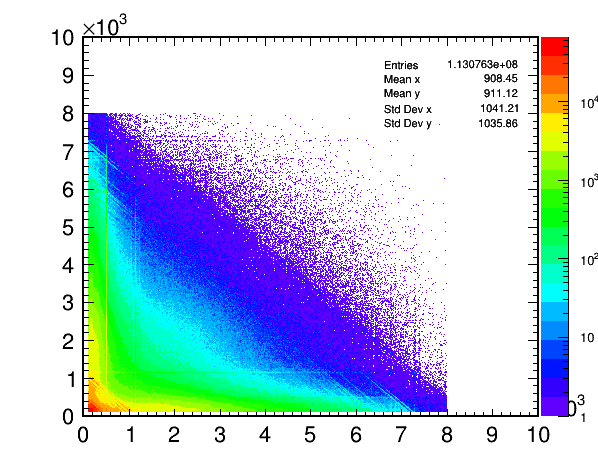
\includegraphics[width=.5\linewidth]{img/155-m1h2.png}
\end{frame}
\begin{frame}[t]{azeazeaze}
\hypertarget{targetname}{}
\fcolorbox{red}{black}{Text mit farbigen Rahmen}
\centering
    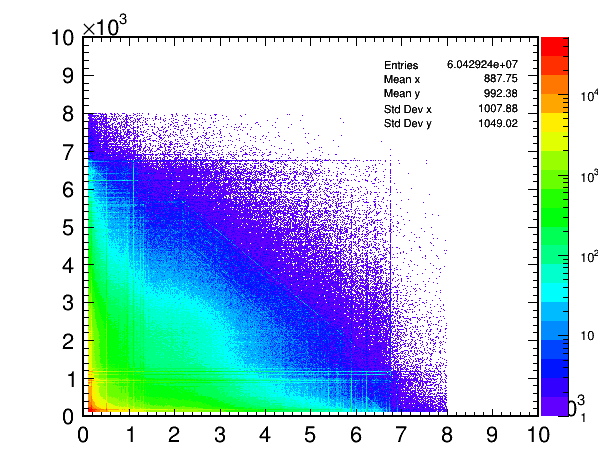
\includegraphics[width=.5\linewidth]{img/157-m2h2.png}
\end{frame}
\endgroup

\subsection{Une longue soussection pour essayer}
\begin{frame}[t]{azeazeaze}
\fcolorbox{red}{black}{Text mit farbigen Rahmen}
\centering
    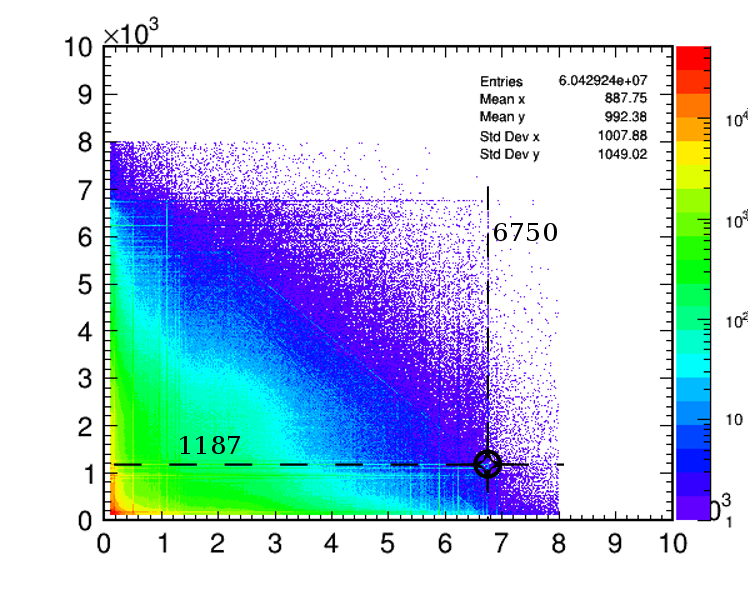
\includegraphics[width=.5\linewidth]{img/157-m2h2a.png}
\end{frame}
\begin{frame}[t]{azeazeaze}
\fcolorbox{red}{black}{Text mit farbigen Rahmen}
\end{frame}

%\end{CJK}
\end{document}